
%%%%%%%%%%%%%%%%%%%%%%%%%%%%%%%%%%%%%%%%%%%%%%%%%%%%%%%%%%%%%%%%%%%%%%%%%%%%%%%%%%%%%%%
%%%%%%%%%%%%%%%%%%%%%%%%%%%%%%%%%%%%%%%%%%%%%%%%%%%%%%%%%%%%%%%%%%%%%%%%%%%%%%%%%%%%%%%
% 
% This top part of the document is called the 'preamble'.  Modify it with caution!
%
% The real document starts below where it says 'The main document starts here'.

\documentclass[12pt]{article}

\usepackage{amssymb,amsmath,amsthm}
\usepackage[top=1in, bottom=1in, left=1.25in, right=1.25in]{geometry}
\usepackage{fancyhdr}
\usepackage{enumerate}
\usepackage{listings}
\usepackage{graphicx}
\usepackage{float}
% Comment the following line to use TeX's default font of Computer Modern.
\usepackage{times,txfonts}



\makeatletter
\renewcommand*\env@matrix[1][*\c@MaxMatrixCols c]{%
  \hskip -\arraycolsep
  \let\@ifnextchar\new@ifnextchar
  \array{#1}}
\makeatother

\newtheoremstyle{homework}% name of the style to be used
  {18pt}% measure of space to leave above the theorem. E.g.: 3pt
  {12pt}% measure of space to leave below the theorem. E.g.: 3pt
  {}% name of font to use in the body of the theorem
  {}% measure of space to indent
  {\bfseries}% name of head font
  {:}% punctuation between head and body
  {2ex}% space after theorem head; " " = normal interword space
  {}% Manually specify head
\theoremstyle{homework} 

% Set up an Exercise environment and a Solution label.
\newtheorem*{exercisecore}{Exercise \@currentlabel}
\newenvironment{exercise}[1]
{\def\@currentlabel{#1}\exercisecore}
{\endexercisecore}

\newcommand{\localhead}[1]{\par\smallskip\noindent\textbf{#1}\nobreak\\}%
\newcommand\solution{\localhead{Solution:}}

%%%%%%%%%%%%%%%%%%%%%%%%%%%%%%%%%%%%%%%%%%%%%%%%%%%%%%%%%%%%%%%%%%%%%%%%
%
% Stuff for getting the name/document date/title across the header
\makeatletter
\RequirePackage{fancyhdr}
\pagestyle{fancy}
\fancyfoot[C]{\ifnum \value{page} > 1\relax\thepage\fi}
\fancyhead[L]{\ifx\@doclabel\@empty\else\@doclabel\fi}
\fancyhead[C]{\ifx\@docdate\@empty\else\@docdate\fi}
\fancyhead[R]{\ifx\@docauthor\@empty\else\@docauthor\fi}
\headheight 15pt

\def\doclabel#1{\gdef\@doclabel{#1}}
\doclabel{Use {\tt\textbackslash doclabel\{MY LABEL\}}.}
\def\docdate#1{\gdef\@docdate{#1}}
\docdate{Use {\tt\textbackslash docdate\{MY DATE\}}.}
\def\docauthor#1{\gdef\@docauthor{#1}}
\docauthor{Use {\tt\textbackslash docauthor\{MY NAME\}}.}
\makeatother

% Shortcuts for blackboard bold number sets (reals, integers, etc.)
\newcommand{\Reals}{\ensuremath{\mathbb R}}
\newcommand{\Nats}{\ensuremath{\mathbb N}}
\newcommand{\Ints}{\ensuremath{\mathbb Z}}
\newcommand{\Rats}{\ensuremath{\mathbb Q}}
\newcommand{\Cplx}{\ensuremath{\mathbb C}}
%% Some equivalents that some people may prefer.
\let\RR\Reals
\let\NN\Nats
\let\II\Ints
\let\CC\Cplx

%%%%%%%%%%%%%%%%%%%%%%%%%%%%%%%%%%%%%%%%%%%%%%%%%%%%%%%%%%%%%%%%%%%%%%%%%%%%%%%%%%%%%%%
%%%%%%%%%%%%%%%%%%%%%%%%%%%%%%%%%%%%%%%%%%%%%%%%%%%%%%%%%%%%%%%%%%%%%%%%%%%%%%%%%%%%%%%
% 
% The main document start here.

% The following commands set up the material that appears in the header.
\doclabel{Math 614: Homework 2}
\docauthor{Stefano Fochesatto}
\docdate{\today}

\begin{document}


\begin{exercise}{P5} This question requires nothing but calculus as a prerequisite. It shows a major source of linear systems from applications.
  \begin{enumerate}[a.]
    \item Consider these three equation, chosen for visualizability:
          \begin{equation*}
            x^2 + y^2 + z^2 = 4
          \end{equation*}
          \begin{equation*}
            x = cos(\pi y)
          \end{equation*}
          \begin{equation*}
            z = y^2
          \end{equation*}
          Provide a sketch of each equation individually as a surface in $\RR^3$. Consider where all three surfaces intersect, describe
          informally why there are two solutions. Explain why both solutions are inside the closed box $-1\leq x \leq 1$, $-2\leq y \leq 2$, and $0\leq z \leq 2$.\\
          \solution First let's consider a graph of each of the surfaces described above.
          \begin{figure}[H]
            \begin{center}
              \caption{The three proposed surfaces.}
              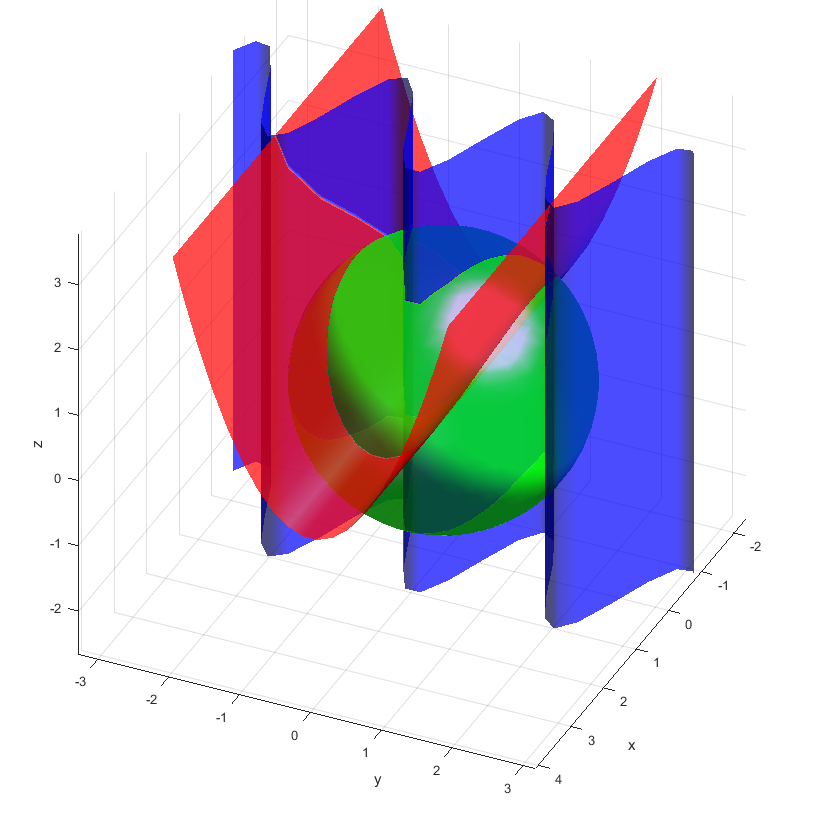
\includegraphics[width=.75\textwidth]{figure1.png}
            \end{center}
          \end{figure}
          \textbf{Code:}
          \begin{center}
            \lstinputlisting{firstplot.txt}
          \end{center}
          Describing the solutions we can see that the ellipsoid and the parabolic cylinder intersect at a curve that looks like a taco shell (Don't know how else to describe the curve).
          When this curve is projected to the $x-y$ plane it only intersects the function $x = cos(\pi y)$ in two places. The solutions lie within $-1\leq x \leq 1$ because we are bounded by $x = cos(\pi y)$,
          $0\leq z$ because we are bounded by $z = y^2$, and $-2\leq y \leq 2$ and $z \leq 2$ because we are bounded by $x^2 + y^2 + z^2 = 4$.
          \vspace{.15in}

    \item Newton's method for a system of nonlinear equations is an iterative, approximate, and sometimes very fast, method for solving systems like the one above. Let $x =(x_1, x_2,x_3) \in \RR^3$.
          Suppose there are three scalar functions $f_i(x)$ forming a column vector function, and consider the system,
          \begin{equation*}
            f(x) = 0,
          \end{equation*}
          Also let,
          \begin{equation*}
            J_{ij} = \dfrac{\delta f_i}{\delta x_j}
          \end{equation*}
          Be the Jacobian matrix: $J \in \RR^{3x3}$. The Jacobian generally depends on location and it generalizes the ordinary scalar derivative.\\
          Newton's method itself is,
          \begin{align}
            J(x_n)s & = -f(x_n) \\
            x_{n+1} & = x_n + s
          \end{align}
          Where $s = (s_1, s_2, s_3)$ is the step and $x_0$ is the initial iterate. Using $x_0 = (-1,1,1)$ write out equation $(1)$ for the $n = 0$ for the surfaces in part $a$,
          as a concrete linear system  of three equation for the three unknown components of step $s = (s_1,s_2,s_3)$. \\
          \solution First let's form the vector function $f(x)$ with the surfaces in part a,
          \begin{equation*}
            f(x) =
            \begin{bmatrix}
              x_1^2 +x_2^2 + x_3^2 - 4 \\
              cos(\pi x_2) -x_1        \\
              x_2^2 - x_3
            \end{bmatrix}
          \end{equation*}
          Now we can consider the associated Jacobian for this system,
          \begin{equation*}
            J(x) = \begin{bmatrix}
              2x_1 & 2x_2              & 2x_3 \\
              -1   & -\pi sin(\pi x_2) & 0    \\
              0    & 2x_2              & -1
            \end{bmatrix}
          \end{equation*}
          Solving each for $x_0 = (-1,1,1)$,
          \begin{equation*}
            f(x_0) =
            \begin{bmatrix}
              -1^2 +1 + 1 - 4 \\
              cos(\pi) -(-1)  \\
              1^2 - 1
            \end{bmatrix}
            =
            \begin{bmatrix}
              -3 \\
              0  \\
              0
            \end{bmatrix}
          \end{equation*}
          \begin{equation*}
            J(x_0) =
            \begin{bmatrix}
              2(-1) & 2(1)          & 2(1) \\
              -1    & -\pi sin(\pi) & 0    \\
              0     & 2(1)          & -1
            \end{bmatrix}
            =
            \begin{bmatrix}
              -2 & 2 & 2  \\
              -1 & 0 & 0  \\
              0  & 2 & -1
            \end{bmatrix}
          \end{equation*}
          Putting everything together to form the system to solve for $s$,
          \begin{equation*}
            \begin{bmatrix}
              -2 & 2 & 2  \\
              -1 & 0 & 0  \\
              0  & 2 & -1
            \end{bmatrix}
            \begin{bmatrix}
              s_1 \\
              s_2 \\
              s_3
            \end{bmatrix}
            = -
            \begin{bmatrix}
              -3 \\
              0  \\
              0
            \end{bmatrix}
          \end{equation*}
          \vspace{.15in}

    \item Implement Newton's method in Matlab to solve the part $(a)$ nonlinear system. Show your script and
          generate at least five iterations. Use $x_0 = (-1,1,1)$ as an initial iterate to find one solution, and
          also find the other solution using a different initial iterate. Note that $format$ $long$ is appropriate here.\\
          \solution
          \textbf{Code:}
          \begin{center}
            \lstinputlisting{NewtonsMethodP5.m}
          \end{center}

          \textbf{Console:}
          \begin{center}
            \lstinputlisting{P5C.txt}
          \end{center}
          \vspace{.15in}

    \item In calculus you likely learned Newton's method as a memorized formula $x_{n+1} =x_n - f(x_n)/f'(x_n)$.
          rewrite equations $(1)$ and $(2)$ for $\RR^1$ to derive this formula.
          \solution  We can see that equation $(1)$ for $\RR^1$ is,
          \begin{equation*}
            f'(x_n)s =-f(x_n).
          \end{equation*}
          We also get that equation $(2)$ for $\RR^1$ is,
          \begin{equation*}
            x_{n+1} = x_n + s
          \end{equation*}
          Solving the first equation for $s$ and substituting into the second equation we get,
          \begin{equation*}
            x_{n+1} = x_n - \dfrac{f(x_n)}{f'(x_n)}
          \end{equation*}
  \end{enumerate}
\end{exercise}
\vspace{.25in}

\begin{exercise}{P6} Its likely that you have learned a recursive method for computing determinants called
  "expansion by minors".
  \begin{enumerate}[a.]
    \item Compute the following determinant by hand to demonstrate that you can apply expansion in minors:
          \begin{equation*}
            \left|\begin{bmatrix}
              1 & 2 & 3 \\
              4 & 5 & 6 \\
              7 & 8 & 9
            \end{bmatrix}\right|
          \end{equation*}
          \solution From what I remember we called this method co-factor expansion,
          \begin{equation*}
            \left|\begin{bmatrix}
              1 & 2 & 3 \\
              4 & 5 & 6 \\
              7 & 8 & 9
            \end{bmatrix}\right|
            = \left|\begin{bmatrix}
              5 & 6 \\
              8 & 9
            \end{bmatrix}\right|
            -2
            \left|\begin{bmatrix}
              4 & 6 \\
              7 & 9
            \end{bmatrix}\right|
            +3
            \left|\begin{bmatrix}
              4 & 5 \\
              7 & 8
            \end{bmatrix}\right|
          \end{equation*}
          \begin{equation*}
            \left|\begin{bmatrix}
              1 & 2 & 3 \\
              4 & 5 & 6 \\
              7 & 8 & 9
            \end{bmatrix}\right|
            = 5*9-8*6
            -2(4*9 - 7*6)
            +3(4*8 - 7*5)
            = 0
          \end{equation*}
          \vspace{.15in}

          \item For any matrix $A \in \CC^{mxm}$, count the exact number of multiplication 
          operations needed to compute the determinant of $A$ with expansion in minors.\\
          \solution Let's first recall the first step to compute the determinant with the expansion in minors method for
          matrix $A$, 
          \begin{equation*}
            det(A) = a_{1,1}*det(A_{m-1,m-1}) - a_{1,2}*det(A_{m-1,m-1}) + \dots a_{1,m}*det(A_{m-1,m-1})
          \end{equation*}
          Now consider forming a recurrence $f(m)$ for counting the number of of multiplications and note that we also know the base case for the 
          recurrence $f(2) = 2$.
          \begin{equation*}
            f(m) = mf(m-1) + m 
          \end{equation*}
          Expanding we get the following, 
          \begin{align*}
            f(m) &= mf(m-1) + m \\
            &= m((m-1)f(m-2) + (m-1)) + m \\
            &= m(m-1)f(m-2) + m(m-1) + m \\
            &= m(m-1)((m-2)f(m-3) + (m-2)) + m(m-1) + m \\
            &= m(m-1)(m-2)f(m-3) + m(m-1)(m-2) + m(m-1) + m \\
            &\dots\\
            &= m(m-1)(m-2)\dots(3)f(2) + \sum_{i = 2}^{m-1} \dfrac{m!}{i!}\\
            &= \dfrac{m!}{2!}f(2) + \sum_{i = 2}^{m-1} \dfrac{m!}{i!}\\
            &= m! + \sum_{i = 2}^{m-1} \dfrac{m!}{i!}
          \end{align*}
          \vspace{.15in}

          \item We know that if $det(A)  = 0$ then $A$ is not invertible. However, rounding error makes an exact
          zero value extremely unlikely. On the other hand, the magnitude of $det(A)$ does not measure invertibility of $A$.
          For instance give a formula for $det(A)$ when $A$ is diagonal and give a formula for $A^{-1}$ if it exists. Show by example that
          $det(A)$ is often very large or very small even for well-conditioned diagonal matrices. \\
          \solution Suppose diagonal matrix $A \in \CC^{mxm}$. Applying the cofactor expansion(expansion by minor) we get the following, 
          \begin{equation*}
            det(A) = a_{1,1}*det(A_{m-1,m-1}) - a_{1,2}*det(A_{m-1,m-1}) + \dots a_{1,m}*det(A_{m-1,m-1})
          \end{equation*}
          Note that only values $A_{i,i}$ will result in non-zero the equation above simplifies greatly, 
          \begin{equation*}
            det(A) = a_{1,1}*det(A_{m-1,m-1})
          \end{equation*}
          Applying this same simplification to each inner determinant we get, 
          \begin{equation}
            det(A) = \prod_{i = 1}^m a_{i,i}.
          \end{equation}
          Suppose this product is non-zero and therefore $A$ is invertible. We know from the matrix multiplication algorithm thant in order to get $A^{-1}A = I$ we need that, 
          \begin{equation*}
            A^{-1} =  \begin{bmatrix}
              \frac{1}{a_{1,1}} & & \\
              & \ddots & \\
              & & \frac{1}{a_{m,m}}
            \end{bmatrix}
          \end{equation*}
          What follows is that, 
          \begin{equation*}
            det(A) = \prod_{i = 1}^m \frac{1}{a_{i,i}}.
          \end{equation*}
          This outlines precisely why we experience rounding error on even the most well conditioned matrices. 
          Consider a large diagonal matrix with extremely large values in the diagonal. From equation 3 we know the resultant determinant 
          will be orders of magnitude larger. Alternatively we know from $4$ that the determinant of the inverse of the matrix 
          will be orders of magnitude smaller. In both cases we experience the limits of IEEE representation. 
  \end{enumerate}
\end{exercise}
\vspace{.5in}

\begin{exercise}{P7} Write a Matlab program which draws the unit balls shown in 3.2 on page 18 of Trefethen
  ann Bau. That is, draw clean pictures of the unit ball of the one, two, infinity, an four norms. \\
  \solution To create each plot I initialized several vectors in 3-space using the 
  sphere command(You could do the same thing with meshgrid command).
  I then coded the norm as an anonymous function (the infinity norm was a little different),
  passing in each vector to compute the magnitude, and then normalizing. What we are left with are unit vectors with respect
  to the corresponding norm. 
  \begin{figure}[H]
    \begin{center}
      \caption{The one-norm unit ball}
      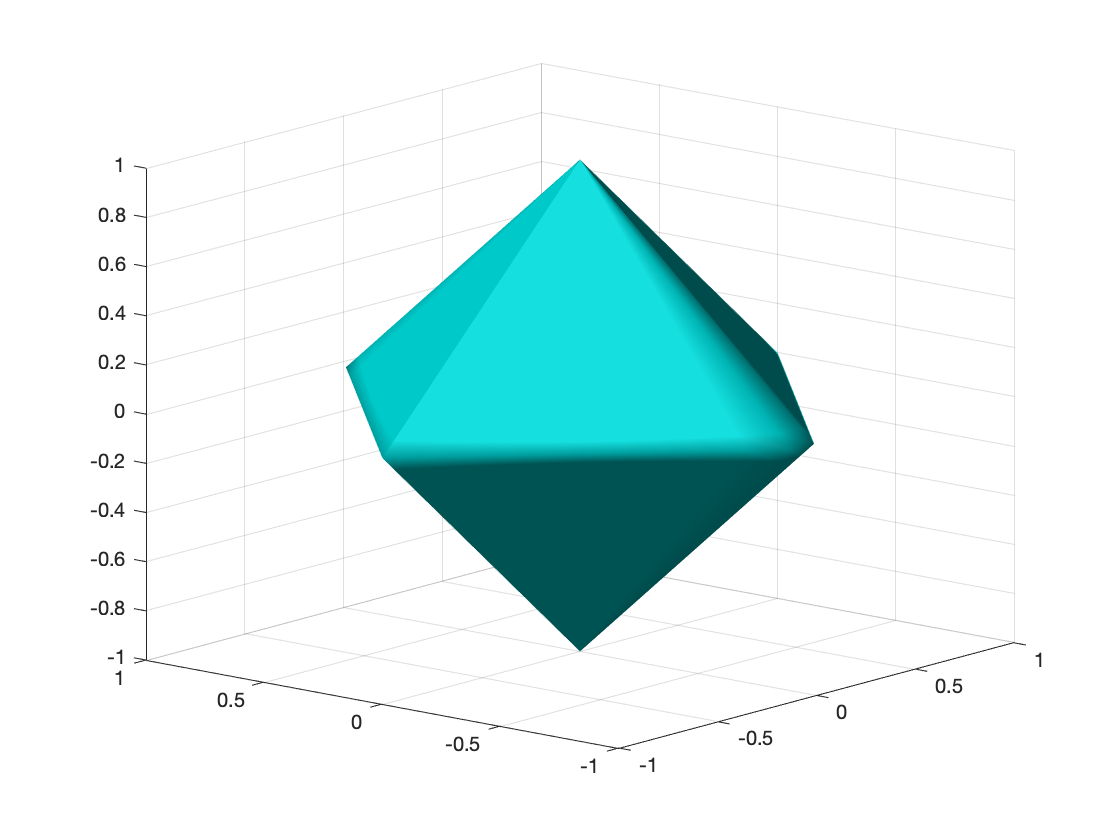
\includegraphics[width=.76\textwidth]{1norm.png}
    \end{center}
  \end{figure}
  \begin{figure}[H]
    \begin{center}
      \caption{The infinity-norm unit ball}
      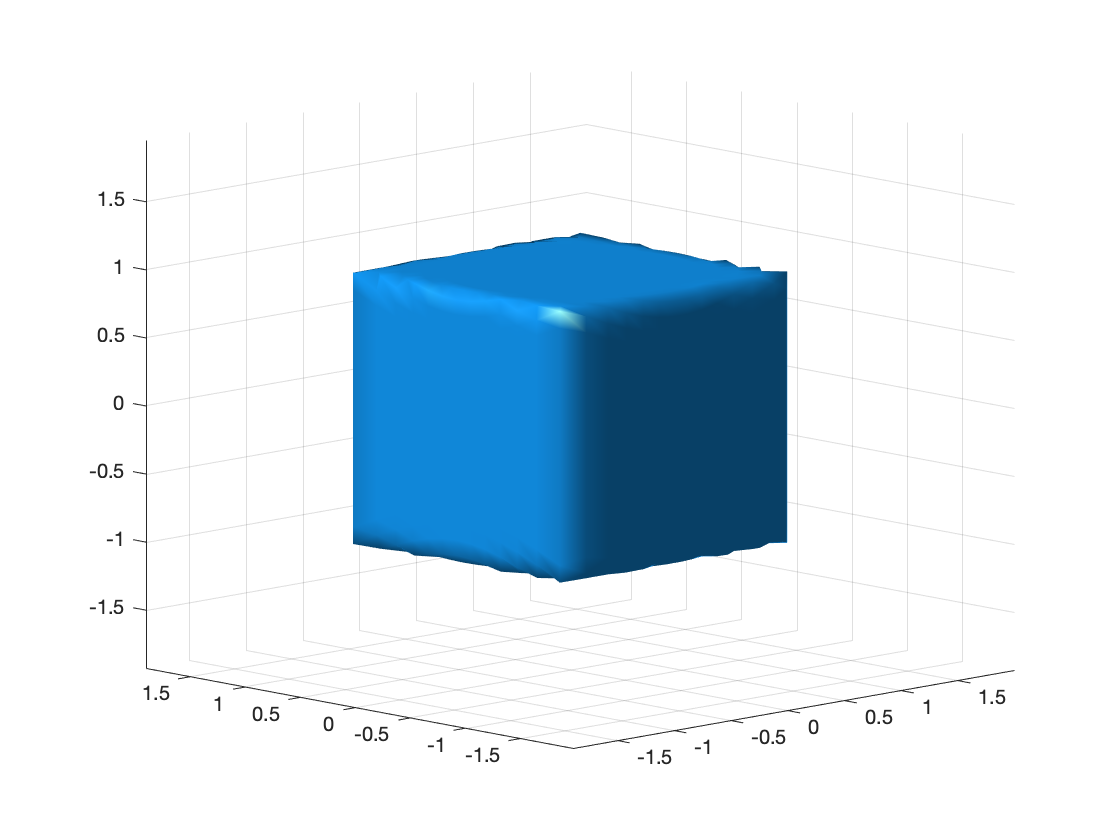
\includegraphics[width=.76\textwidth]{InfNorm.png}
    \end{center}
  \end{figure}
  \begin{figure}[H]
    \begin{center}
      \caption{The two-norm unit ball}
      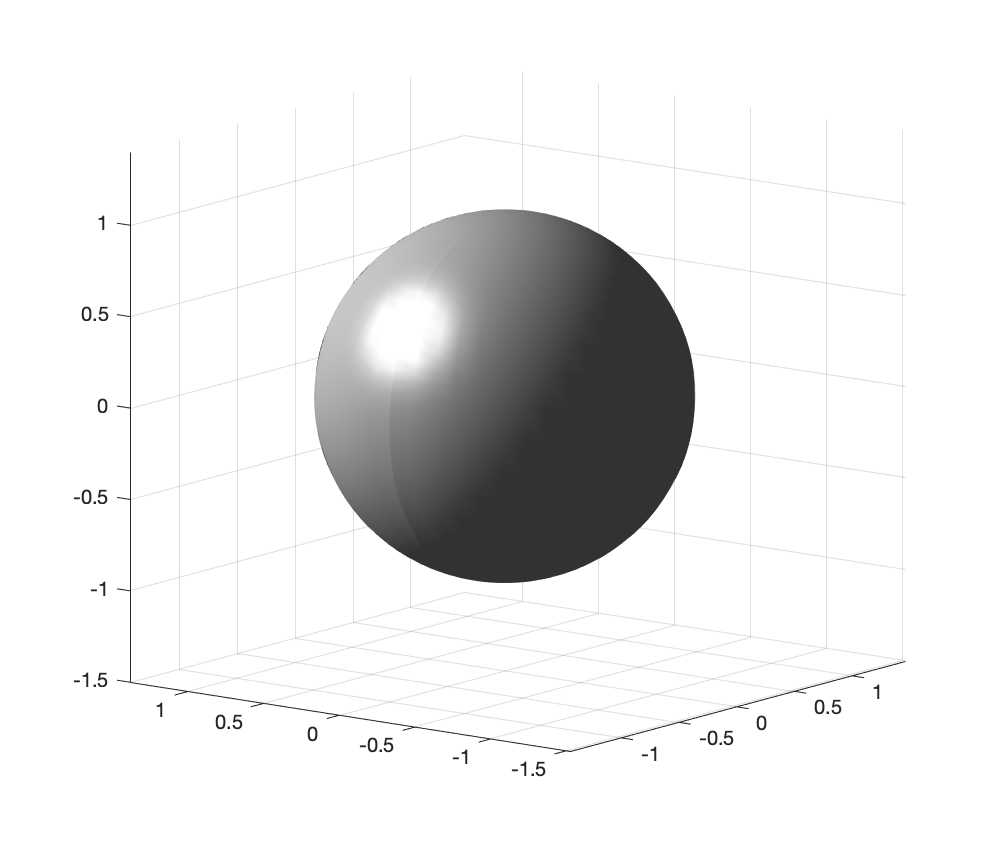
\includegraphics[width=.76\textwidth]{2Norm.png}
    \end{center}
  \end{figure}
  \begin{figure}[H]
    \begin{center}
      \caption{The four-norm unit ball}
      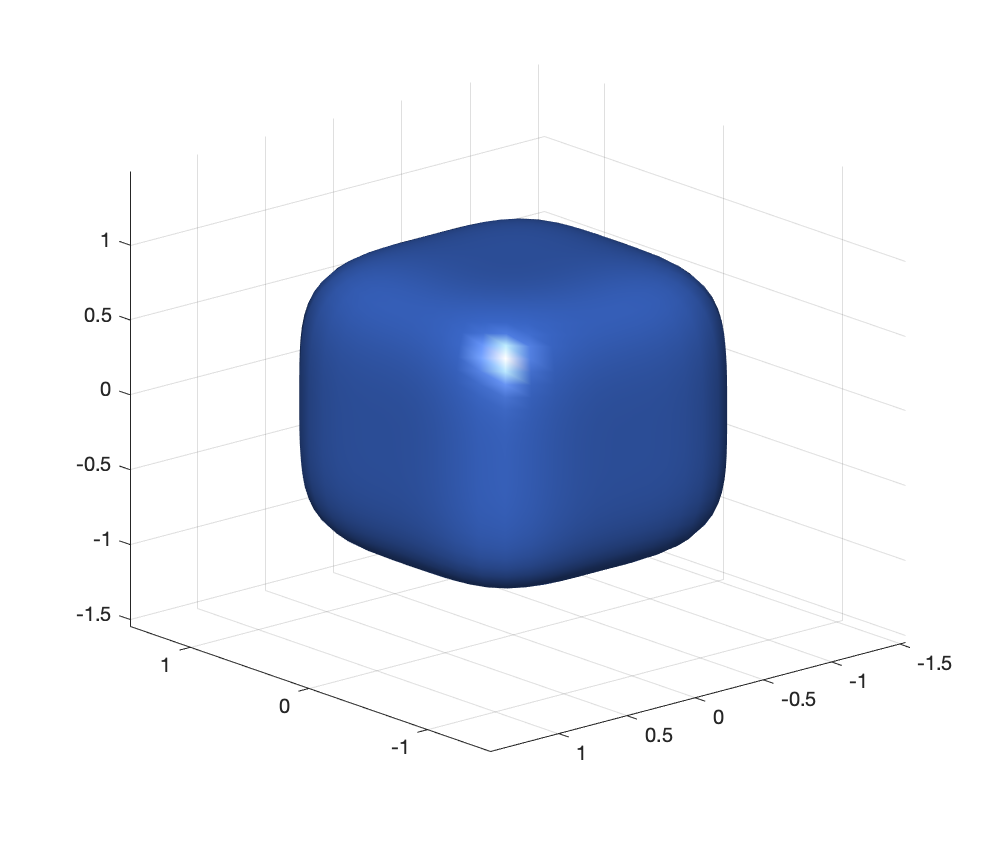
\includegraphics[width=.76\textwidth]{4Norm.png}
    \end{center}
  \end{figure}
  \textbf{Code:}
  \begin{center}
    \lstinputlisting{Norm.m}
  \end{center}
\end{exercise}

\vspace{.25in}

\begin{exercise}{2.1} Show that if a matrix is both triangular and unitary then it 
  must be diagonal.\\
  \solution Suppose a matrix $A$ is both triangular and unitary. By the definition of unitary we know that 
  \begin{equation*}
    A^*A = I. 
  \end{equation*}
  Or equivalently, 
  \begin{equation*}
    A^* = A^{-1}. 
  \end{equation*}
  Let's assume without loss of generality that $A$ is upper triangular. Recall that since $A$ is an upper triangular matrix then $A^{-1}$ must also be upper triangular (exercise 1.3).
  Clearly if $A$ was not diagonal, $A^*$ would be lower triangular and $A^{-1}$ would be upper triangular, therefore 
  it follows that $A$ must be diagonal. 
\end{exercise}

\vspace{.25in}

\newpage
\begin{exercise}{2.3} Let $A \in \CC^{mxm}$ be hermitian. An eigenvector of $A$ is a nonzero vector
  $x \in \CC^m$ such that $Ax = \lambda x$ for some $\lambda \in \CC$ the corresponding eigenvalue. 
  \begin{enumerate}[a.] 
    \item Prove that all eigenvalues of $A$ are real.\\
    \solution Suppose that $A \in \CC^{mxm}$ is hermitian and consider that for some eigenvector and eigenvalue $x, \lambda$ we have the following,
    \begin{equation*}
      Ax = \lambda x.
    \end{equation*}
    Left multiplying both sides by the $x^*$ we get the following,
    \begin{align*}
      x^*Ax &= x^*\lambda x\\
       &= \lambda x^*x\\
       &= \lambda ||x||^2
    \end{align*}
    Now consider taking the adjoint of both sides.
    \begin{align*}
      (x^*Ax)^* &= (\lambda ||x||^2)^*\\
      x^*A^*x &= \bar{\lambda} ||x||^2
    \end{align*}
    Since $A$ is hermitian we know that $A^* = A$. Therefore by substitution we get, 
    \begin{equation*}
      x^*Ax = \bar{\lambda} ||x||^2
    \end{equation*}
    Note that by substituting $x^*Ax$ we can say that, 
    \begin{equation*}
      \lambda ||x||^2 = \bar{\lambda} ||x||^2
    \end{equation*}
    We know that $||x||^2$ must always be non-zero since it is defined by a non-zero eigenvector. 
    Dividing both sides by $||x||^2$ we are left with $\lambda = \bar{\lambda}$ which is only possible when $\lambda$ is a real number.

    \vspace{.15in}

    \item Prove that if $x$ and $y$ are eigenvectors corresponding to distinct eigenvalues 
    then $x$ and $y$ are orthogonal. \\
    \solution Suppose $A$ is hermitian with eigenvectors $x$ and $y$ and their corresponding eigenvalues $\lambda_x$ and 
    $\lambda_y$. By definition we know that, 
    \begin{equation}
      Ax = \lambda_xx
    \end{equation}
    \begin{equation}
      Ay = \lambda_yy
    \end{equation}
    Taking equation 4, left multiplying $y^*$, and simplifying similarly to the last problem we get, 
    \begin{align*}
      y^*Ax &= y^* \lambda_xx,\\
      &=  \lambda_x y^*x,\\
      &=  \lambda_x <x,y>.
    \end{align*}
    Taking equation 5, left multiplying $x^*$, and simplifying similarly to the last problem we get, 
    \begin{align*}
      x^*Ay &= x^* \lambda_yy,\\
      &=  \lambda_y y^*x,\\
      &=  \lambda_y <x,y>.
    \end{align*}
    Taking the adjoint of both sides we get, 
    \begin{align*}
      (x^*Ay)^* &= \bar{\lambda_y} <x,y>,\\
      (Ay)^*x &= \bar{\lambda_y} <x,y>,\\
      y^*A^*x &= \bar{\lambda_y} <x,y>.
    \end{align*}
    Since $A$ is hermitian, by substitution we get that,
    \begin{equation*}
      y^*Ax = \bar{\lambda_y} <x,y>.
    \end{equation*}
    Substituting $y^*Ax$ and with some algebra we can see that,
    \begin{align*}
      \lambda_x <x,y> &= \bar{\lambda_y} <x,y>,\\
      \lambda_x <x,y> - \bar{\lambda_y} <x,y> &= 0,\\
      <x,y>(\lambda_x - \bar{\lambda_y}) &= 0.
    \end{align*}
    Since we know that $\lambda_x$ and $\bar{\lambda_y}$ are distinct real values it must be the case that 
    $<x,y> = 0$ and therefore $x$ and $y$ are orthogonal. 
    \vspace{.15in}
  \end{enumerate} 

\end{exercise}



\end{document}




















